% Homework report template for courses lectured by Blaz Zupan.
% For more on LaTeX please consult its documentation pages, or
% read tutorials like http://tobi.oetiker.ch/lshort/lshort.pdf.
%
% Use pdflatex to produce a PDF of a report.

\documentclass[a4paper,11pt]{article}
\usepackage{a4wide}
\usepackage{fullpage}
\usepackage[toc,page]{appendix}
\usepackage[pdftex]{graphicx} % for figures
\usepackage{setspace}
\usepackage{color}
\definecolor{light-gray}{gray}{0.95}
\usepackage{listings} % for inclusion of Python code
\usepackage{hyperref}
\renewcommand{\baselinestretch}{1.2}

\lstset{ % style for Python code, improve if needed
language=Python,
basicstyle=\footnotesize,
basicstyle=\ttfamily\footnotesize\setstretch{1},
backgroundcolor=\color{light-gray},
}

\title{Mario}
\author{Zidar Miha (63060317)}
\date{\today}

\begin{document}

\maketitle

\section{Introduction}

In this report we will present the results of Q learning for Super Mario from 12th rl competition 2009.


\section{Methods}

For learning we used a simple Q matrix, where states were represented as strings surrounding Mario. To make monsters more important, we clipped the string to just have Mario and the nearest monster. For each step we propagated the reward back with the function:

\begin{equation} \label{eq1}
Q[s][a] = Q[s][a] + \frac{reward}{ 1 + offset from current action / 10} 
\end{equation}

This proved to be much better than the original formula:

\begin{equation} \label{eq2}
Q[s][a] = Q[s][a] + \alpha * (reward + \gamma * Q[s'][a'] - Q[s][a])
\end{equation}

\section{Results}

\begin{figure}[htbp]
    \begin{center}
        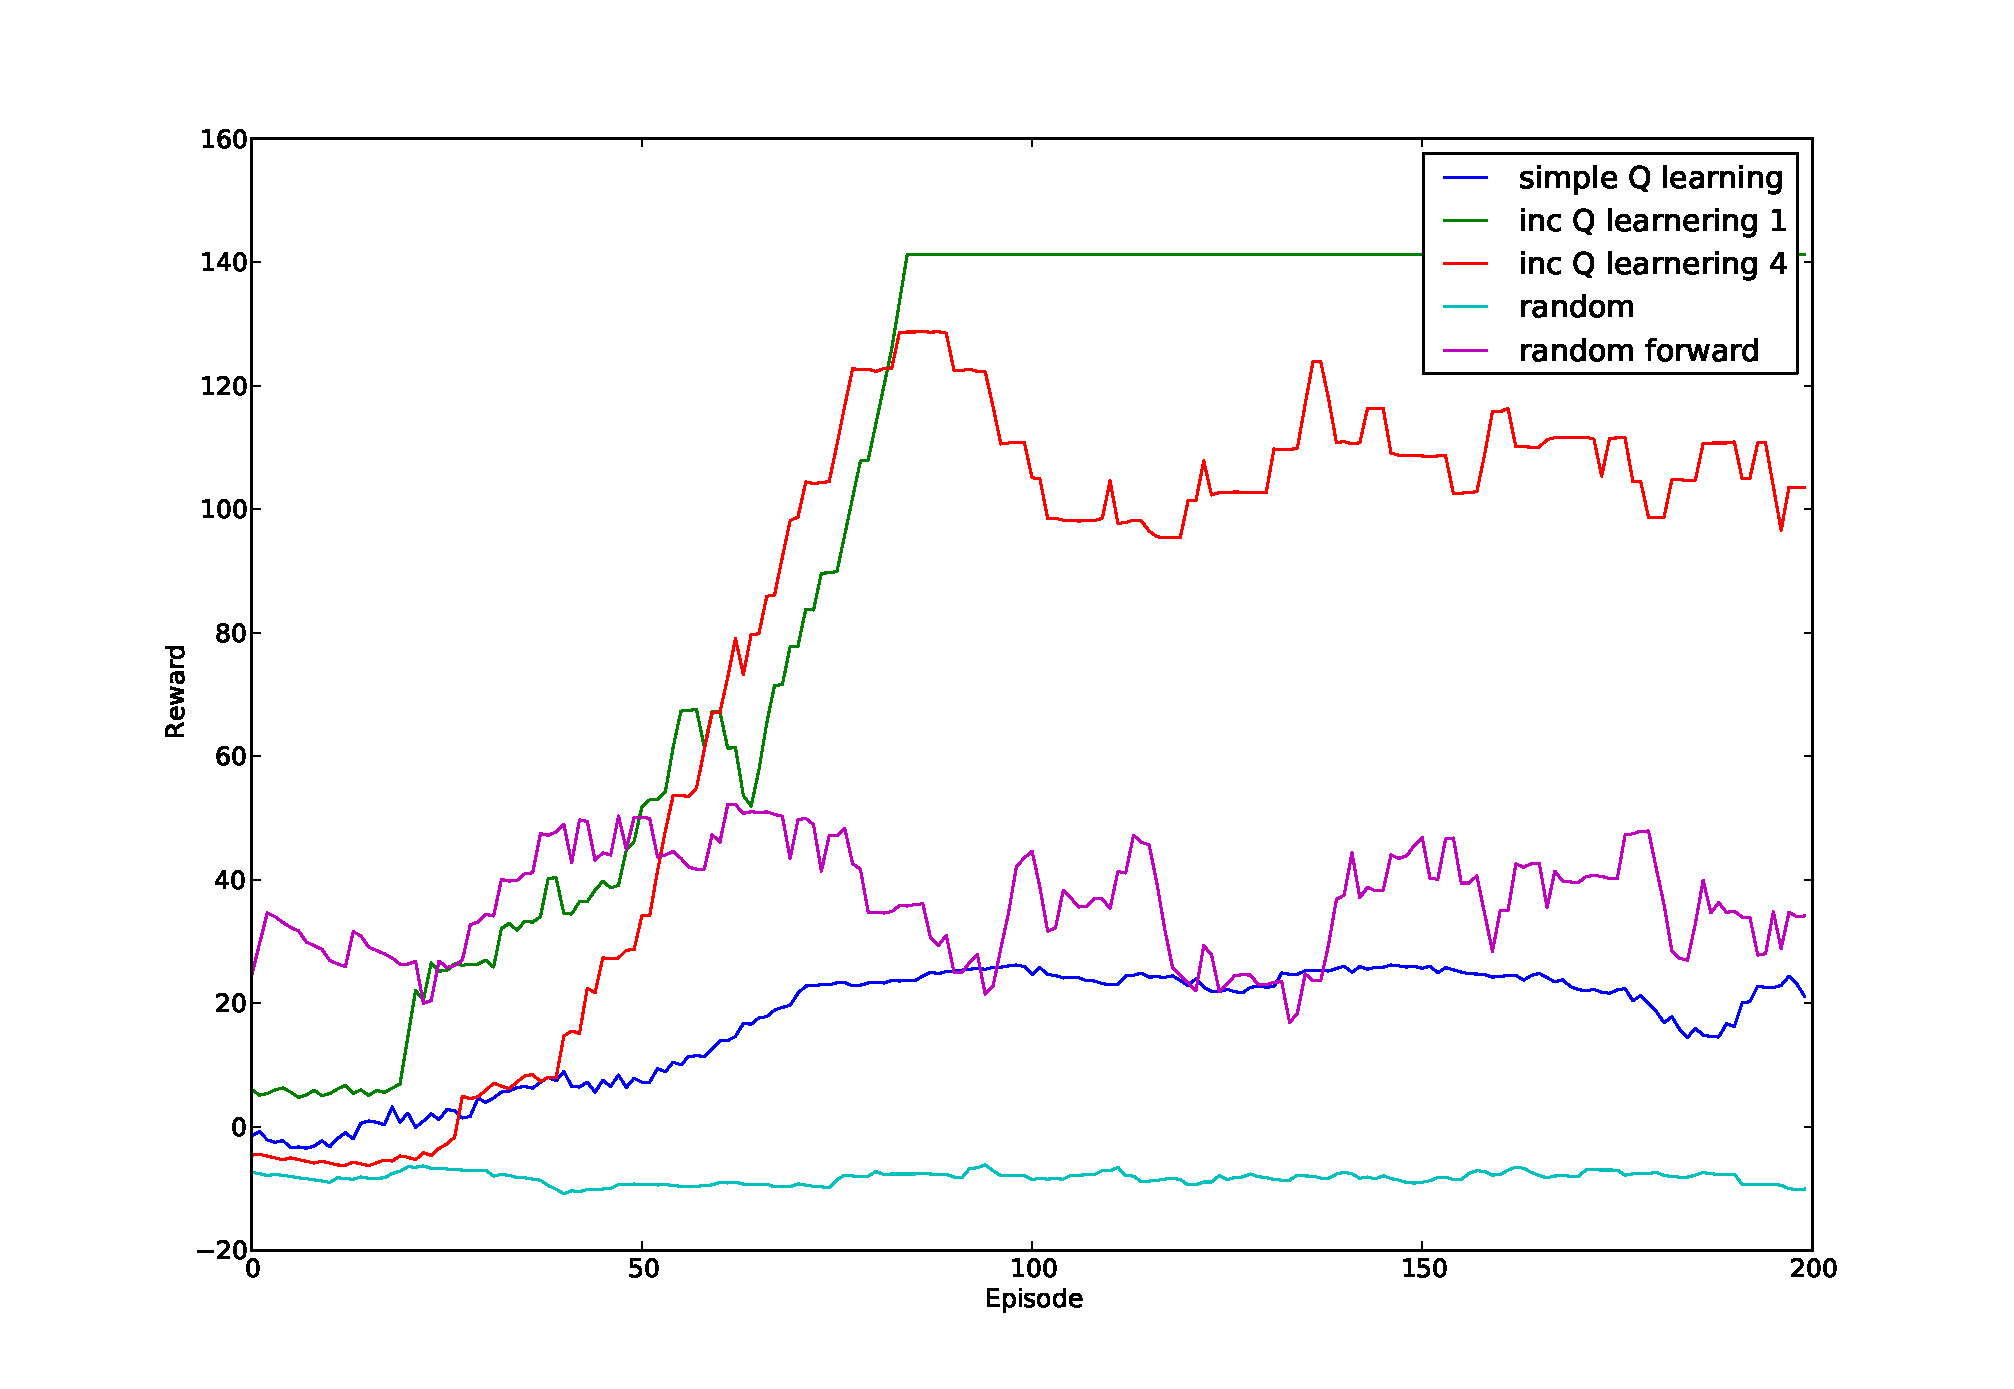
\includegraphics[scale=0.4]{graph.pdf}
        \caption{Result of learning with 200 trials}
        \label{graph}
    \end{center}
\end{figure}



Here we have the result of the previously mentioned algorithm, and control runs.

\begin{itemize}
    \item random - selects all actions randomly.
    \item random forward - selects all actions randomly, but without the option to go back.
    \item simple Q learning - Q learning with equation \ref{eq2}
    \item inc Q learning 1 - same as above but with equation \ref{eq1} and with all movements set to run, thus reducing the action space from 12 actions to possible 6 actions.
    \item inc Q learning 2 - same as Q learning 1, but with full movement set, and added option of exploration once a good method has been found.
\end{itemize}





\end{document}

